\documentclass[11pt]{beamer}
\mode<presentation>{
\usetheme{Madrid}
\setbeamercovered{transparent}
}

\usepackage[slovak]{babel}
\usepackage[utf8]{inputenc}
\usepackage{amsmath}
\usepackage{amsthm}
\usepackage{amsfonts}
\usepackage[IL2]{fontenc}
\usepackage{graphicx}
\usepackage{lmodern}
\usepackage{hyperref}

\newtheorem{formal}{Formálna definícia}

\title{Konečné automaty}
\author{Sabína Gregušová}
\institute[xgregu02]{\\Vysoké učenie technické v~Brne \\Fakulta informačních technológií\\ \medskip \texttt{xgregu02@stud.fit.vutbr.cz}}
\date{\scriptsize{4. 5. 2018}}


\begin{document}
\begin{frame}
\titlepage
\end{frame}

\begin{frame}{Základné informácie}
\textbf{Konečný automat} (anglicky finite state machine) je výpočetný model primitívneho počítača, ktorý sa skladá z~viacerých stavov a prechodov. \vspace{0.5cm}

Najpoužívanejšie sú:
\begin{itemize}
\item Konečný automat typu Moore,
\item Konečný automat typu Mealy.
\end{itemize}
\vspace{0.5cm}
Pre grafické znázornenie prechodov sa používa \textbf{stavový diagram}. 
\end{frame}

\begin{frame}{Konečný automat typu Moore}
\begin{formal} 
Je to usporiadaná šestica $(X, Y, S, S_0, \delta, \omega)$, kde: 
\\$X : | X | < \infty$ je konečná vstupná abeceda,
\\$Y : | Y | < \infty$ je konečná výstupná abeceda,
\\$S : | S | < \infty$ je konečná množina vnútorných stavov,
\\$S_0 : S_0 \in S$ je východzí vnútorný stav,
\\$ \delta : S\times X \rightarrow S$ je priechodová funkcia,
\\$ \omega : S \rightarrow Y$ je výstupná funkcia.
\end{formal}
\end{frame}
\begin{frame}{Čo to znamená?}
Každý vnútorný stav má definovanú práve jednu hodnotu na výstupe. Automat musí mať definovaný
východzí vnútorný stav, v~ktorom sa nachádza pred zadaním prvého vstupného symbolu a pravidlá pre prechody
medzi jednotlivými stavmi.
\begin{figure}[h]
\begin{center}
\scalebox{0.3}{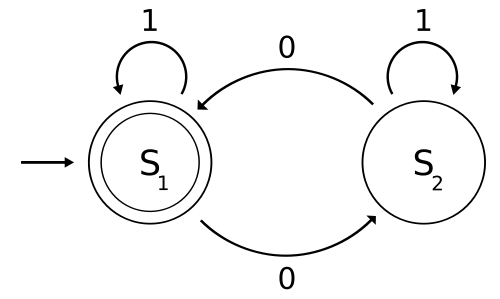
\includegraphics{moore.png}}
\caption{Ilustračný diagram konečného automatu Moore}
\end{center}
\end{figure}
\end{frame}

\begin{frame}{Konečný automat typu Mealy}
\begin{formal} 
Je to usporiadaná šestica $(X, Y, S, S_0, \delta, \omega)$, kde: 
\\ $X : | X | < \infty $ je konečná vstupná abeceda,
\\ $Y : | Y | < \infty$ je konečná výstupná abeceda,
\\ $S : | S | < \infty$ je konečná množina vnútorných stavov,
\\ $S_0 : S_0 \in S$ je východzí vnútorný stav,
\\ $ \delta : S \times X \rightarrow S $ je priechodová funkcia,
\\ $ \omega : S \times X \rightarrow Y$ je výstupná funkcia.
\end{formal}
\end{frame}

\begin{frame}{Čo to znamená?}
Mealy je vo svojej podstate iba zobecnením typu Moore. Hlavný rozdiel je, že výstup nezávisí len na vnútornom stave, ale aj na výstupe. Vo formálnej definícii sa táto odlišnosť prejavuje iným definičným oborom výstupnej funkcie. Do vystupnej funkcie vstupuje ako parameter aj aktuálny prvok vstupnej abecedy.
\begin{figure}[h]
\scalebox{0.05}{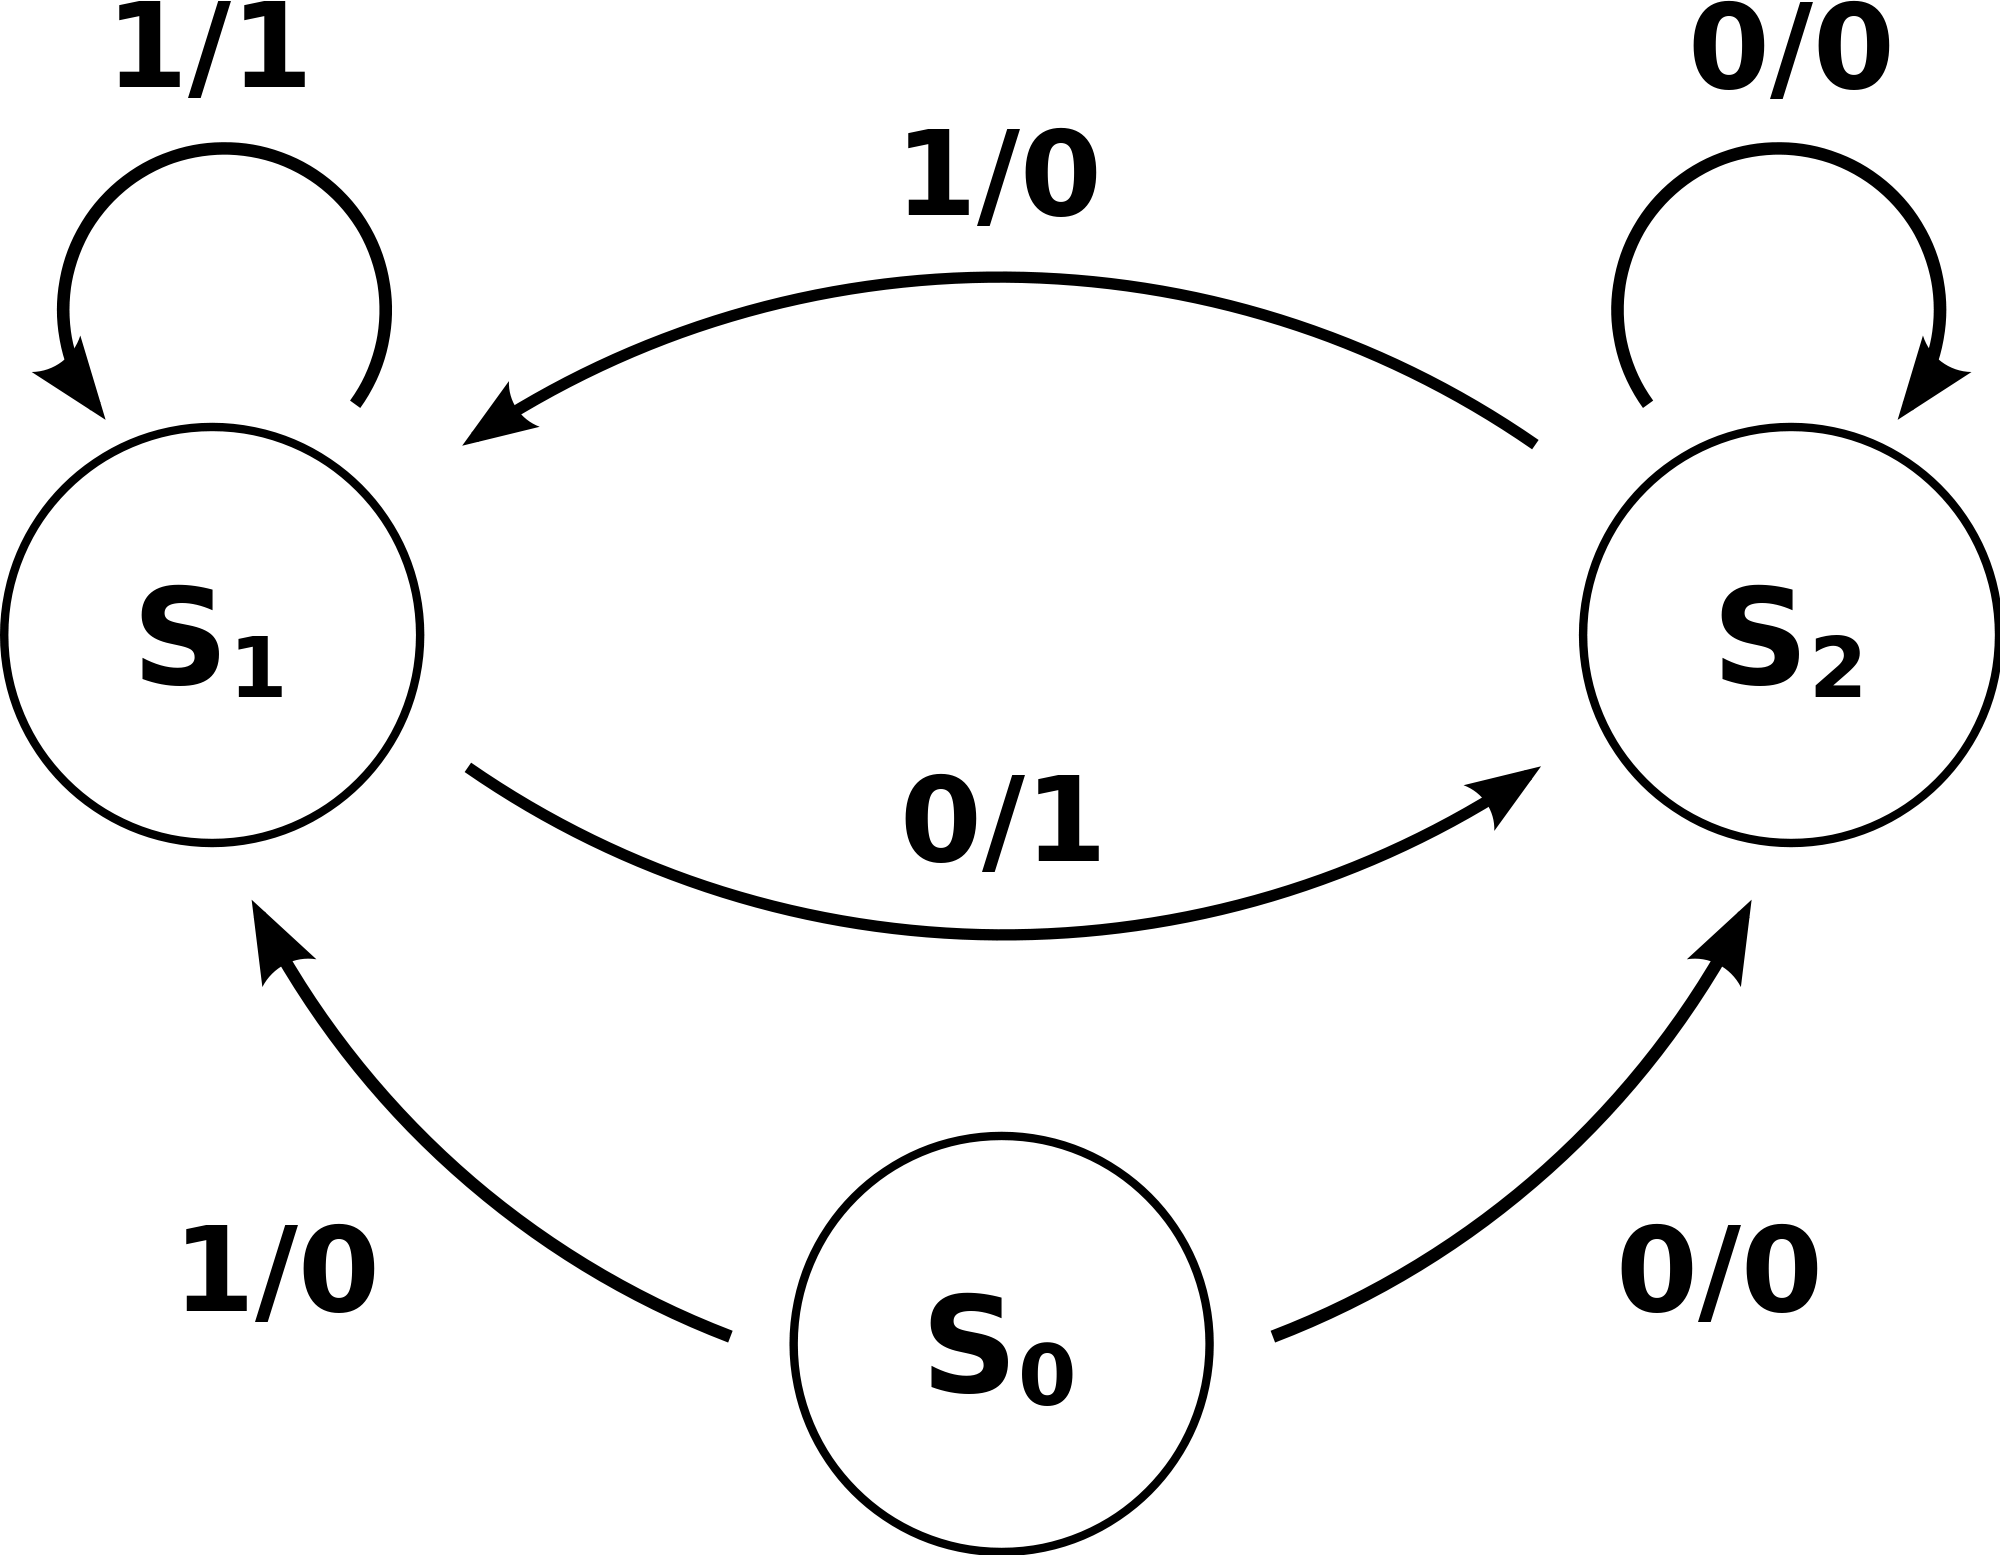
\includegraphics{mealy.png}}
\caption{Ilustračný diagram konečného automatu Mealy}
\end{figure}
\end{frame}

\begin{frame}{Použité zdroje}
\begin{itemize}
\item Diagramy\\ \vspace{0.5mm}
{\footnotesize \url{http://masters.donntu.org/2007/fvti/ykubovskyy/library/state_diagram-Wikipedia.htm}}
\item Konečný automat typu Mealy\\ \vspace{0.5mm}
{\footnotesize \url{http://voho.eu/wiki/mealy/}}
\item Konečný automat typu Moore\\ \vspace{0.5mm}
{\footnotesize \url{http://voho.eu/wiki/moore/}}
\item Konečný automat\\ \vspace{0.5mm}
{\footnotesize \url{https://matematika.cz/konecny-automat}}
\end{itemize}
\end{frame}


\end{document}